\documentclass[espaco=simples,appendix=Name]{abnt}
\usepackage[utf8]{inputenc}
\usepackage[brazil]{babel}
\usepackage{hyperref}
\usepackage[alf]{abntcite}
\usepackage{mdwlist}
\usepackage{dsfont}
\usepackage{graphicx}
\usepackage{float}
\def\Data$#1 #2 #3${#2}

\autor{Matheus Eduardo B. Morais e Bruno Rubin}
\titulo{Suporte a Codificação e Decodificação do WebP no Mozilla Firefox}
\orientador{Isabel H. Manssour}
\instituicao{Pontifícia Universidade Católica do Rio Grande do Sul (PUCRS)}
\local{Porto Alegre}
\data{\Data$Date: 2012/08/28 $}
\begin{document}
\capa
\folhaderosto
\sumario

\newcommand{\ingles}[1]{\textsl{#1}}
\newcommand{\bibTeX}{bib\kern-.13ex\TeX}

\chapter{Introdução}

\begin{description}

\section{Contextualização}

\item \noindent A internet se resume nos dias de hoje ao chamado WWW, ou \ingles{World Wide Web} onde usuários acessam páginas da \ingles{Web} escritas em uma linguagem específica definida por uma organização internacional (W3C), que é renderizada através de um software chamado de navegador. O usuário então pode ler as informações descritas ali e acessar os demais conteúdos da página através de seus hiperlinks de uma maneira fácil e intuitiva.

Com a crescente evolução dos meios de comunicação, a necessidade de total interatividade do usuário com as páginas aumentou cada vez mais. Uma página da \ingles{Web} não é somente texto como era nos primórdios, ela é composta de uma série de diferentes atores como folhas de estilo, imagens e vídeos. Estes atores existem para aumentar a facilidade no uso e causar uma experiência mais agradável para o usuário final.

Apesar da mudança na necessidade dos usuários da \ingles{Web}, nenhuma alteração significativa foi feita nos protocolos e linguagens que são utilizadas hoje. Boa parte da tecnologia implementada atualmente foi criada no início dos anos 90 e apesar de sofrerem revisões periódicas, continuam não atendendo totalmente as demandas que surgem. Outro fator importante é que mesmo com o advento nas tecnologias de comunicação, nem todas as pessoas tem acesso a esta evolução. Seja por uma questão econômica ou mesmo pela falta de infraestrutura, nem toda população do planeta pode contar com aquilo que há de mais moderno.

Recentemente a empresa estadunidense \ingles{Google Inc.} promoveu uma série de iniciativas em conjunto com a comunidade internacional no esforço chamado de "\ingles{Let's make the Web Faster}" \cite{WebFaster}, que consiste em um processo de reengenharia dos protocolos, linguagens e demais itens que compõem a \ingles{Web}. Dentro deste processo novos padrões e formatos estão sendo sugeridos para melhorar a performance e a qualidade na experiência do usuário com as páginas. Uma das sugestões é a utilização de um novo método para compressão de imagens chamado de \ingles{WebP}\cite{WebPConcept}. Entretanto, até o presente momento, o suporte a renderização de imagens \ingles{WebP} foi implementado apenas para os navegadores Chrome e Opera.

\section{Motivação}

\item \noindent Os estudos mais recentes mostram que a capacidade de compressão do formato \ingles{WebP} tem cerca de 39\% de ganho quando comparado com JPEG e JPEG200. A Figura 1.1 apresenta um gráfico que ilustra o ganho na porcentagem de compressão.

\begin{figure}[H]
  \centering
    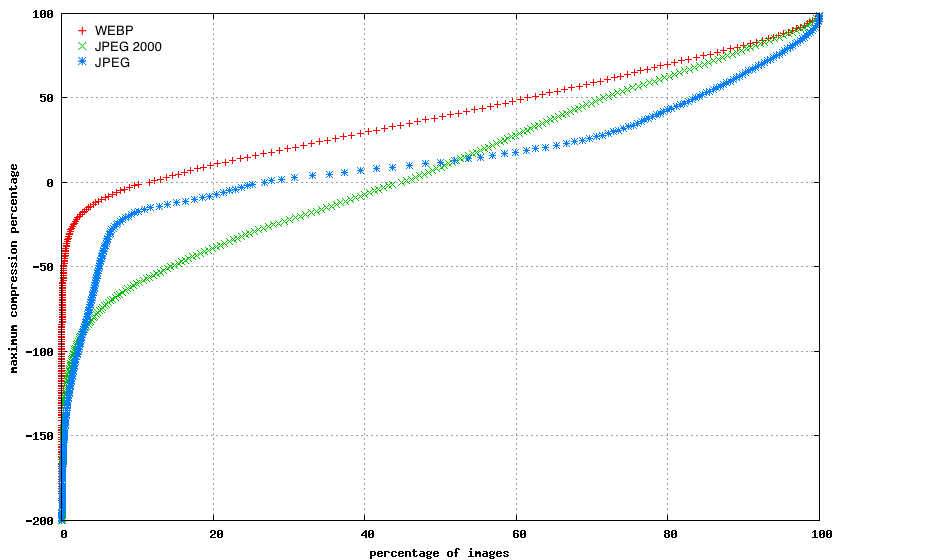
\includegraphics[width=0.9\textwidth]{Plot3_cdfcompr.png}
  \caption{Comparação do tamanho das imagens e porcentagem de compressão \protect\cite{WebPStudy}}
\end{figure}

Embora a implementação do suporte ao \ingles{WebP} esteja somente disponível para dois navegadores (Chrome e Opera), estes constituem mais de 29\% de todos os navegadores utilizados dentro da internet hoje. Se houvesse suporte ao \ingles{WebP} dentro do Mozilla Firefox este percentua aumentaria para 52\%, já que cerca de 22\% dos navegadores utilizados hoje são Mozilla Firefox \cite{BrowserStats}, como ilustra a Figura 1.2.

\begin{figure}[H]
  \centering
    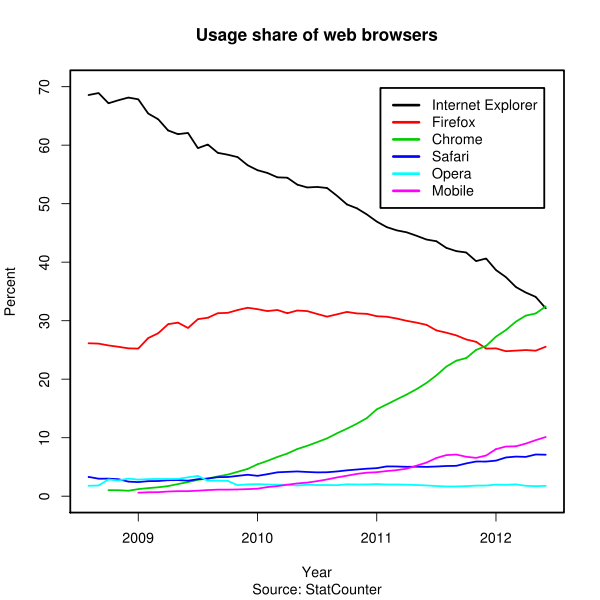
\includegraphics[width=0.6\textwidth]{BrowserCounter.png}
  \caption{Percentual de utilização dos Navegadores na Web \protect\cite{BrowserStats}}
\end{figure}

Embora não exista nenhuma diretiva da W3C para qual método de compressão de imagens utilizar por padrão e não se sabe se haverá tal tipo de registro neste sentido no futuro, é importante ressaltar que quanto mais navegadores suportarem a compressão usando o formato \ingles{WebP}, mais os desenvolvedores vão optar por utilizar este formato dada suas vantagens. Uma força de 52\% de suporte dentro dos navegadores da internet também fará com que aqueles que ainda não decidiram pela implementação do suporte ao novo formato, também o faça em virtude da pressão exercida pela maioria.

O aumento na capacidade de compressão do formato \ingles{WebP} trará de imediato a melhora no tempo de resposta para o \ingles{download} da imagem no navegador do usuário e também diminuirá o trafego na comunicação entre cliente e servidor. É importante notar que a utilização em massa deste novo formato vai ajudar na diminuição do trafego de rede dentro da internet de uma maneira global, e isso resulta diretamente em maior vazão para outros recursos que consomem mais banda, como é o caso de um \ingles{streaming} de vídeo por exemplo.

\section{Objetivo}

\item \noindent
Considerando as vantagens no uso do novo formato \ingles{WebP}, o objetivo deste trabalho é aumentar a sua disseminação dentro da \ingles{Web} através da implementação do suporte à codificação e decodificação do \ingles{WebP} para o navegador Mozilla Firefox. Os benefícios na utilização deste novo formato vão desde de aumento na performance de renderização da página até a redução do trafego de pacotes TCP dentro da internet uma vez que o formato \ingles{WebP} proporciona imagens que são consideravelmente menores do que aquelas utilizadas atualmente. 

\end{description}

\chapter{Fundamentação Teórica}

\begin{description}

\section{A World Wide Web}

\item \noindent
A internet hoje em dia se fundamenta nos princípios da \ingles{World Wide Web} ou somente \ingles{Web} como é conhecida, os usuários se conectam na rede mundial de computadores e utilizam as páginas da \ingles{Web} para realizar todo e qualquer tipo de ação dentro da rede. Desde conversar com seus amigos e familiares até realizar compras em uma página de \ingles{e-commerce}, tudo isso passa pela \ingles{Web}. A \ingles{World Wide Web} foi inventada no CERN, o Centro Europeu de Pesquisa Nuclear, com o principal objetivo de servir como suporte para a consulta e comunicação interna dos projetos de pesquisa do CERN \cite{WebStory}. A ideia era utilizar hipertextos que podiam funcionar também como hiperlinks e faziam ligações para outras páginas com mais informações. Toda plataforma desenvolvida internamente dentro do CERN para a \ingles{Web} foi mais tarde disponibilizada ao domínio público sem cobrança de royalties sob qualquer parte. Mais tarde Tim Berners-Lee, o fundador da \ingles{Web} dentro do CERN, criou a o \ingles{World Wide Web Consortium} com o principal objetivo de definir os padrões utilizados dentro da rede. Conhecido também como W3C, é composto por funcionários de diversas empresas que trabalham em período integral para manter e evoluir os padrões especificados pela organização \cite{W3Cfacts}.

Além de ser utilizada por pessoas, a \ingles{Web} também é utilizada hoje para comunicação entre sistemas. São efetivamente computadores acessando outros computadores para trocarem informações. Como os padrões definidos tem sua especificação aberta, a \ingles{Web} também se torna uma ótima ferramenta para integrar sistemas diferentes em plataformas diferentes. Hoje em dia os chamados \ingles{Web-Services} são utilizados juntamente com os conceitos de Orientação a Objetos para integração entre sistemas. A comunicação utilizando os \ingles{Web-Services} se baseiam nos princípios e padrões especificados pelo W3C para a \ingles{Web} \cite{WebServices}.

Uma parte importante da \ingles{Web} são os chamados \ingles{Web Browsers} ou Navegadores que servem para que as páginas da \ingles{Web} possam ser acessadas e operadas. Os navegadores são ferramentas que interpretam os padrões descritos pela W3C e fazem a interface para que os humanos consigam entender as informações descritas nas páginas e consigam navegar por elas de forma intuitiva, utilizando os hiperlinks.

Com o advento da qualidade na comunicação da internet, as páginas da Web se tornaram cada vez mais elaboradas e interativas. Hoje não são apenas hipertextos com hiperlinks, são sistemas complexos que processam até som, imagem e vídeo. Embora estas funcionalidades dinâmicas existam, não há um padrão claro a respeito dele. A HTML que é a linguagem de programação da Web não oferece um suporte nativo para todas estas implementações e plugins adicionais não padronizados são utilizados para implementar estas necessidades específicas (o Flash Player e o Java FX são um exemplo).

A W3C trabalha em uma evolução da linguagem HTML mais preparada para este tipo de cenário, a chamada HTML5. Dentro da HTML5 existem vários detalhes em discussão e um dos mais importantes é a questão da forma como vídeo e imagem vão ser interpretados. O valor 5 da HTML vem por essa ser a quinta revisão completa da linguagem, que promete ser uma das maiores revisões feitas até hoje \cite{HTML5spec}.

\section{Os Web Browsers}

\item \noindent
Na computação, um \ingles{Web Browser}, também chamado de Navegador, é um \ingles{software} com uma interface gráfica que possui como principal funcionalidade a apresentação de documentos virtuais da Internet, popularmente chamado de páginas da \ingles{Web}, escritos nas linguagens HTML, PHP e ASP, e podendo ser também arquivos PDF, imagens e outros tipos. O \ingles{Web Browser} É destinado principalmente para navegação na \ingles{World Wide Web}, possibilitanto ao usuário uma interação com a informação e o conteúdo publicado. O \ingles{Web Browser} surgiu juntamente com a dissminação da \ingles{World Wide Web}, que necessitava de uma ferramenta apropriada para realizar a busca das informações que estavam disponíveis na grande rede. \cite{ArchitectureWebBrowsers}

Os navegadores, basicamente realizam a comunicação com servidores \ingles{web} através do protocolo de comunicação HTTP. A partir de uma URL (\ingles{Uniform Resource Locator)} informada, é feita a requisição do documento (página) para o servidor, que processa a requisição e retorna a resposta para o navegador, na qual a exibe para o usuário. O navegador é responsável por efetuar a renderização do documento recebido, transformando-o de uma linguagem de marcação (HTML) para um documento interativo.\cite{ArchitectureWebBrowsers}

Com a explosão da utilização da \ingles{Web} na década de 90 \cite{BloombergGameChangers}, diversas grandes empresas da computação, como Microsoft, Google e Apple, investiram no desenvolvimento de novos navegadores para a Internet. Nos dias de hoje, existem cinco principais navegadores utilizados mundialmente, são eles: Microsoft Internet Explorer (Microsoft), Mozilla Firefox (Mozilla Corporation \& Mozilla Foundation), Safari (Apple), Google Chrome (Google) e Opera (Opera Software).

A concorrência existente entre as empresas e os produtos oferecidos atualmente, se dá principalmente pela velocidade de navegação e a utilização dos recursos computacionais. Cada dia mais, surgem novos padrões e estudos de novas tecnologias relacionadas, que possibilitam que os navegadores tenham um melhor desempenho na execução da suas funções. Como exemplo do HTML5, na qual tem como objetivo tornar o conteúdo das páginas mais dinâmico, deixando de lado o conceito do browser que apenas realiza a apresentação do documento, mas que interaja como uma aplicação única através dos recursos e ferramentas. \cite{WebAppPlataform}

\section{HTML5}

\item \noindent
Em 1998 o W3C decidiu que eles não iriam mais continuar o desenvolvimento da linguagem da \ingles{Web} até então, a HTML \ingles{(HyperText Markup Language)}. Ao invés disto eles iriam trabalhar em um novo formato o qual acreditavam ser o futuro da \ingles{Web}, assim nasceu a linguagem XHTML \ingles{(Extensible HyperText Markup Language)} que se fundamentava nos princípios da XML \ingles{(Extensible Markup Language)}. Desta forma a revisão 4.01 da HTML foi congelada e os esforços se direcionaram para a evolução da XHTML que em sua versão 2.0 trazia além de muitas mudanças revolucionárias, a quebra de toda compatibilidade das aplicações escritas nas versões anteriores da especificação.

Muitos não gostaram desta nova iniciativa, em particular um grupo que trabalhava no desenvolvimento do navegador Opera, que não ficou parado e além de não adotar a XHTML começou a trabalhar na especificação de uma linguagem HTML extensiva que não quebrasse a compatibilidade das versões anteriores.  A especificação foi inicialmente chamada de \ingles{Web Forms} 2.0 e mais tarde foi nomeada com HTML5 por ser a quinta revisão da HTML \cite{HTML5Intro}. O W3C então começou a trabalhar na quinta revisão e apesar de não ter sido lançada nenhuma versão final da especificação, praticamente todos navegadores já implementam o suporte à nova definição da HTML.

Uma das necessidades que a HTML5 deve suprir é o suporte para processamento de vídeo e som que nos dias de hoje se fundamenta no \ingles{plugin Flash}. Para esta implementação foi escolhido o formato WebM que possibilita aos navegadores renderizar nativamente vídeo e áudio sem a necessidade de \ingles{plugins} adicionais. O formato WebM é composto pelo método de compressão de vídeo VP8 e o padrão de áudio Vorbis. O WebP é parte integrante do WebM só que com foco voltado para compressão de imagens.

\section{WebP}

\item \noindent
O WebP é um novo formato de imagem que implementa compressão \ingles{lossless} e \ingles{lossy} para imagens na \ingles{Web}. Utilizando uma técnica de compressão \ingles{lossless} o WebP consegue apresentar imagens 26\% menores no tamanho quando comparado com o formato PNG. Utilizando imagens com \ingles{lossy} os resultados são ainda melhores reduzindo de 25-34\% quando comparado com o formato JPEG. O WebP também fornece suporte a transparência com apenas 22\% de \ingles{bytes} adicionais. O WebP utiliza uma metodologia semelhante aquela usada na compressão VP8 que faz parte do pacote WebM para o processamento de vídeo e áudio \cite{WebPLossyStudy}.

A tecnologia por trás do WebP é fundamentada no conceito de \ingles{block prediction}. Cada bloco tem seu valor previsto baseado nos três blocos acima dele e no primeiro bloco a esquerda dele. Existem quatro métodos para previsão dos blocos, a horizontal, a vertical, a DC e a \ingles{TrueMotion}. As informações que foram previstas incorretamente e os blocos que não são previsíveis são comprimidos em um sub-bloco de 4x4 \ingles{pixels}. No final o resultado é comprimido utilizando \ingles{Entropy encoding} que é um método \ingles{lossless} para compressão de dados.

O suporte à codificação e decodificação do WebP está disponível nos navegadores Google Chrome e Opera. Como o Mozilla Firefox já possui suporte ao WebM, alguma parte do código para a implementação do WebP já reside dentro do navegador uma vez que tanto WebP quanto VP8 utilizam a mesma técnica para a compressão de imagens.

\section{Mozilla Firefox e o WebP}

\item \noindent

O formato WebP foi disponibilizado em 2010 mas nunca conseguiu ser integrado ao Mozilla Firefox. Inclusive na época um \ingles{bug} foi aberto dentro do \ingles{bugzilla} da Mozilla solicitando a implementação do formato WebP \cite{FirefoxBug}. Naquela tempo a equipe principal de desenvolvimento do Mozilla Firefox decidiu por não realizar a implementação em virtude de uma série de considerações contrárias ao formato WebP \cite{WebPCritica}. O time de desenvolvimento do WebP levou em conta as críticas que recebeu dos desenvolvedores do Mozilla Firefox e fez uma série de ajustes para suprir as necessidades que estavam sendo demandadas. Embora praticamente todos os apontamentos dados tenham sido ajustados ainda não há uma clara razão do por que ele ainda não foi implementado. Em 2010 um \ingles{patch} rudimentar foi escrito e submetido mas não foi aceito. Existem também algumas extensões que fazem com que o Firefox consiga exibir imagens WebP, porem estas extensões não caracterizam um desenvolvimento adequado visto que elas dependem de plugins adicionais. A proposta é que o navegador seja capaz de realizar a codificação e decodificação nativamente. 

Pelo que parece há por trás disso uma razão política na não adoção do formato WebP até o presente momento. Apesar do Google ter aumentado os investimentos no desenvolvimento do Mozilla Firefox em 2011, o Google Chrome vem tomando espaço do Firefox na internet e há um temor de que a própria existência do Firefox esteja ameaçada graças ao grande sucesso do navegador concorrente. Entretanto pelo que foi pesquisado dentro da comunidade há alguma chance de que caso uma implementação decente seja feita, ela poderá ser aceita dentro do código oficial.

\end{description}

\chapter{Trabalhos Relacionados}

\begin{description}

\item \noindent
Os seguintes trabalhos estão relacionados com o tema proposto:

\begin{itemize}
%	\item x264 Biblioteca para codificação e decodificação de imagem e áudio.
	\item JPEG 2000 Atualização do padrão JPEG para compressão de imagens.
	\item JPEG XR Alternativa mais leve ao JPEG 2000 para compressão de imagens.
\end{itemize}

%\section{Biblioteca x264}
\section{JPEG 2000}
JPEG 2000 é um padrão de compressão de imagens, criado pela Joint Photographic Experts Group com o objetivo de ser amplamente utilizado em diversas áreas. Suas principais aplicações se deram em câmeras digitais, possibilitando imagens com resoluções maiores, de maior qualidade, utilizando uma compressão dessas informações em um arquivo fisicamente menor; na \ingles{Internet}; em impressões avançadas; em imagens médicas e outros setores chaves. O objetivo do JPEG 2000 não é apenas melhorar o desempenho de compressão em relação ao JPEG, mas adicionar (ou melhorar) características como escalabilidade e capacidade de edição.

O formato JPEG 2000 trouxe alguns benefícios em relação ao JPEG, sendo eles:
\begin{itemize}
	\item Compressão da imagem sem perda de qualidade
	\item Preservação da transparência nas imagens
	\item Uso de máscaras (canais alpha) para especificar uma área da imagem que necessite ser salva em uma taxa de compressão mais baixa (perda de informação de imagem) do que outras áreas que possui um menor interesse para o usuário
	\item Preservação das informações EXIF nos arquivos de imagem
	\item Opções do usuário quanto ao tamanho, qualidade e número de imagem de visualização-miniaturas em um site.
\end{itemize}

A principal vantagem oferecida pelo formato JPEG 2000 é a flexibilidade no manuseio do codestream obtido após uma compressão de imagem utilizando este algoritmo. O codestream obtido, pode ser descodificado de diversas maneiras.

O JPEG 2000 foi publicado como um padrão ISO, ISO / IEC 15444. Atualmente o formato não é suportado em navegadores web e, portanto, não é geralmente utilizado na \ingles{Internet}.\cite{JPEG}

\section{JPEG XR}
O formato de imagem JPEG XR (abreviação para \ingles{JPEG extended range}) é um padrão de compressão de imagens desenvolvido e patenteado pela Microsoft sob o nome de HD Photo.
Com a a popularidade do formato JPEG 2000 em baixa, devido à pouco suporte de aplicativos e falta de melhorias no formato, a Microsoft desenvolveu o JPEG XR, na qual se diz comparável com o JPEG 2000, e mais eficiente que o JPEG. Ao contrário do JPEG 2000, este novo formato proposto pela Microsoft é proprietário, ou seja, necessita de drivers e \ingles{plug-ins} específicos para codificação e decodificação das imagens em plataformas que ainda não possui suporte nativo.

O formato JPEG XR suporta a compressão de imagens com e sem perda de qualidade. Em relação ao JPEG original, oferece várias melhorias-chave, como:
\begin{itemize}
\item Melhor compressão dos dados
\item Compressão sem perda de qualidade
\item Suporte de cores com maior precisão
\item Suporte a  mapeamento de transparência
\item Suporte a metadados
\end{itemize}

Atualmente o JPEG XR é suportado por diversas aplicações Adobe Flash Player 11.0, Adobe AIR 3.0, Sumatra PDF 2.1, Windows Imaging Component, .NET Framework 3.0, Windows Vista, Windows 7, Windows 8, Internet Explorer 9, Internet Explorer 10, porém não é comumente utilizado em sites da \ingles{Internet}.\cite{HDPhoto}

\end{description}

\chapter{Proposta}
\begin{description}

\section{Objetivos}

\item \noindent
Conforme apresentado na seção 1.3, o objetivo deste trabalho visa contribuir com o desenvolvimento de uma solução para codificação e decodificação do formato de imagem WebP para o browser Mozilla Firefox. 
A motivação do desenvolvimento desta solução, conforme descrito na seção 1.2, se dá pelo fato de que o formato WebP já se encontrar em um estado avançado de desenvolvimento e maturidade, e já estar recebendo suporte nativo dos browsers Google Chrome e Opera. 

O aumento na capacidade de compressão do formato \ingles{WebP} trará de imediato a melhora no tempo de resposta para o \ingles{download} da imagem no navegador do usuário e também diminuirá o trafego na comunicação entre cliente e servidor. É importante ressaltar também que a popularização e utilização em massa deste novo formato irá beneficiar na diminuição do trafego de rede dentro da internet de uma maneira global, e isso resulta diretamente em uma vazão maior para outros recursos que consomem mais banda, como é o caso de um \ingles{streaming} de vídeo por exemplo.

\section{Ambiente de Desenvolvimento}

\item \noindent
Para montagem do ambiente de desenvolvimento será necessário realizar o \ingles{checkout} de todo código fonte do Mozilla Firefox a partir do CVS oficial pois o trabalho será realizado em cima de classes e métodos já existentes. O navegador é desenvolvido utilizando a linguagem de programação C++, por tanto está será a linguagem na qual o trabalho será desenvolvido. Deverá ser feita uma análise para identificar a necessidade de reescrever a biblioteca \ingles{WebP} de acordo com a sua especificação ou se poderá haver um reaproveitamento de código da implementação que já existe.

\chapter{Recursos Necessários}
A seguir serão apresentados os recursos mínimos de \ingles{hardware} e \ingles{software} necessários para o desenvolvimento do trabalho proposto.

\section{Recursos de Hardware}
\begin{itemize}
	\item Dell Intel Core I5 @ 2,50GHz 4 GB Ram
	\item Macbook Pro Core 2 Duo @ 2,53GHz 8 GB Ram	
\end{itemize}
	
\section{Recursos de Software}
\begin{itemize}
	\item Mac OS X Lion
	\item Debian GNU/Linux
	\item Xcode
	\item Biblioteca \LaTeX
	\item Biblioteca \bibTeX
	\item Biblioteca WebP
	\item Código fonte do Mozilla Firefox
	\item Git
	\item VIM
	\item GCC
	\item GNU Make
\end{itemize}

\end{description}

\chapter{Tarefas a serem desenvolvidas}

\begin{description}
\item \noindent
Neste capítulo serão descritas as tarefas que devem ser realizadas no decorrer do trabalho bem como um cronograma detalhando os prazos no qual cada atividade será executada.

\section{Atividades}
\begin{itemize}
        \item Estudo da biblioteca e do formato WebP.
        \item Estudo e detalhamento do código do Mozilla Firefox para renderização de imagens.
        \item Estudo e detalhamento dos padrões de codificação do Mozilla Firefox.
        \item Modelagem das classes para codificação e decodificação a partir dos estudos realizados.
        \item Desenvolvimento da documentação para o trabalho final.

\end{itemize}
\section{Cronograma}
\begin{figure}[H]
  \centering
    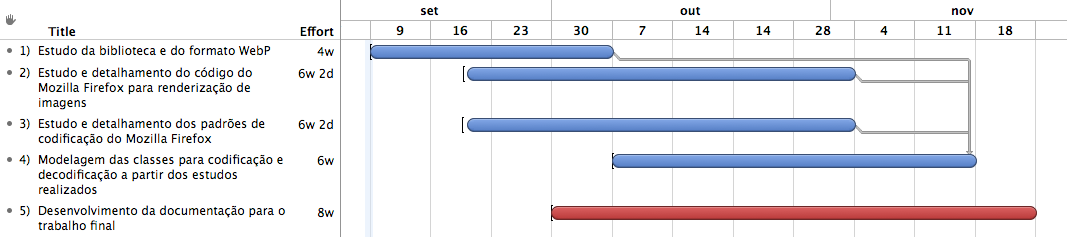
\includegraphics[width=0.9\textwidth]{scheduler.png}
  \caption{Planejamento das atividades para desenvolvimento do trabalho}
\end{figure}
\end{description}

\bibliography{proposta}

\end{document}
